%*-------------------------------------------------------------------------*
%*                 Copyright 2013-2015 Core Physics, Inc.                  *
%*  Under terms of the contract to support CASL, there is a non-exclusive  *
%*  license for use of this work by or on behalf of the U.S. Government.   *
%*-------------------------------------------------------------------------*
%
% @version CVS $Id: core.tex,v 1.12 2015/02/23 00:52:46 scott Exp $
%
%%%%%%%%%%%%%%%%%%%%%%%%%%%%%%%
\subsection{Core Description}

The [CORE] block describes the nuclear reactor core configuration. This block describes the core layout, including
the placement of nuclear fuel assemblies, control rods, detectors, inserts, and other core parameters
that do not change during a cycle depletion.

The geometric objects inside the core are defined in separate input blocks; the [CORE] block
simply describes how all of these objects are placed together.

\subsubsection{Core Geometry}

The reactor core geometry must be defined first. The overall {\it size} of the core is
given by the number of assemblies across one major axis of the core. The assembly pitch ({\it apitch}) defines the
width of each assembly, including the assembly gap. The distance from the top of the lower core plate to the
bottom of the upper core plate is given by the parameter {\it height}.
The assembly layout is given by the {\it core\_shape} map.
Note that the core shape map is the only ``square'' core map in the input, and it must be of {\it size} assemblies by {\it size}.
Once the core shape is defined, subsequent core maps only include entries for actual fuel assembly locations.

\begin{Verbatim}[fontsize=\small]

  size 15            ! number of assemblies across one axis
  apitch 21.5        ! assembly pitch (cm)
  height 406.337     ! distance from lower core plate to upper core plate (cm)

  core_shape
    0 0 0 0 1 1 1 1 1 1 1 0 0 0 0
    0 0 1 1 1 1 1 1 1 1 1 1 1 0 0
    0 1 1 1 1 1 1 1 1 1 1 1 1 1 0
    0 1 1 1 1 1 1 1 1 1 1 1 1 1 0
    1 1 1 1 1 1 1 1 1 1 1 1 1 1 1
    1 1 1 1 1 1 1 1 1 1 1 1 1 1 1
    1 1 1 1 1 1 1 1 1 1 1 1 1 1 1
    1 1 1 1 1 1 1 1 1 1 1 1 1 1 1
    1 1 1 1 1 1 1 1 1 1 1 1 1 1 1
    1 1 1 1 1 1 1 1 1 1 1 1 1 1 1
    1 1 1 1 1 1 1 1 1 1 1 1 1 1 1
    0 1 1 1 1 1 1 1 1 1 1 1 1 1 0
    0 1 1 1 1 1 1 1 1 1 1 1 1 1 0
    0 0 1 1 1 1 1 1 1 1 1 1 1 0 0
    0 0 0 0 1 1 1 1 1 1 1 0 0 0 0

\end{Verbatim}

The {\it core\_shape} map is unique because it is square in shape and composed of the integers 1 and 0.
The 1 represents a location with a fuel assembly, and a 0 is an unoccupied location.
The purpose of this map is to define the shape for subsequent core maps.

Most physics codes support calculations run in either full-core, half-core, or quarter-core symmetry.
If a calculation is run in half-core or quarter-core symmetry, the code must know whether the symmetry is
mirror symmetric or rotationally symmetric. The type of symmetry is defined with the {\it bc\_sym}
input card. The symmetry option is ignored if the calculation is run in full-core.
\begin{Verbatim}[fontsize=\small]
  bc_sym mir    ! define quarter-core symmetry as mirror

\end{Verbatim}

\subsubsection{Core Maps}

Core maps are used to define the location of geometry objects in the core.
There are different core maps to define types and locations of assemblies,
inserts, detectors, and control rods.
The entries in the maps are composed of arbitrary-length character strings.
Even though the character strings can be any size, it is recommended to use
compact names so the maps remain legible.

All of the maps require one entry for each assembly location defined in the {\it core\_shape} map.
However, the input parser can be used to take advantage of core symmetry. If the core is symmetric, then
the user only needs to input the maps in quarter or octant symmetry, and the input parser will automatically
unfold the map to full symmetry using mirror symmetry, regardless of the value for {\it bc\_sym}.
The symmetry used in the core maps is independent of the symmetry used to run the actual calculations.
For example, the user can enter all of the core maps in octant symmetry and still run the calculations
in quarter or full symmetry.
The quadrant and octant that the parser expects is shown in Figure~\ref{fig:coresym}.

\begin{figure}[hbt!]
\begin{center}
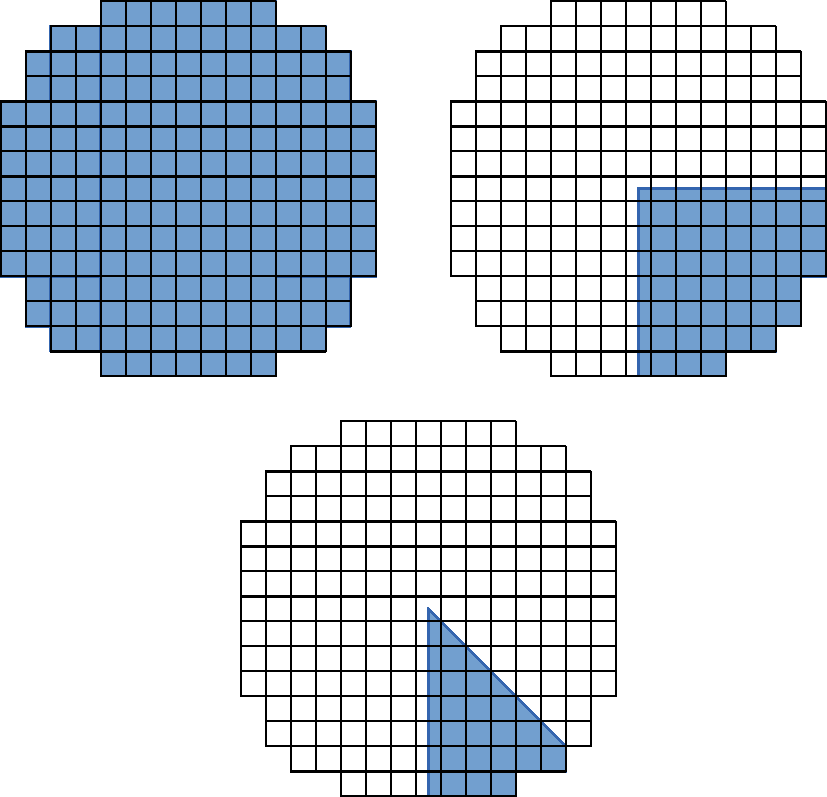
\includegraphics[width=5in]{figs/core_symmetry.pdf}
\end{center}
\caption{\label{fig:coresym} Full, quarter, and octant symmetry regions for a core map.}
\end{figure}

If there is an empty location in the map (e.g., if there is no detector or no control rod
in an assembly), then enter a dash (also known as a \textit{hyphen}) ``-'' for that location. The dash is significant and signifies an
empty location in the core map. (The dash indicates that something is missing, but it is still
a valid assembly location. The ``0'' in the {\it core\_shape} represents an invalid assembly location.)


\clearpage

The {\it assm\_map} shows where the assembly types are located within the core.
In the example below, there are three assembly types that will be defined in [ASSEMBLY] block(s).
\begin{Verbatim}[fontsize=\small]

  assm_map
                  A3 A3 A3 A3 A3 A3 A3
            A3 A3 A3 A1 A3 A1 A3 A1 A3 A3 A3
         A3 A3 A2 A1 A2 A1 A2 A1 A2 A1 A2 A3 A3
         A3 A2 A2 A2 A1 A2 A1 A2 A1 A2 A2 A2 A3
      A3 A3 A1 A2 A1 A2 A1 A2 A1 A2 A1 A2 A1 A3 A3
      A3 A1 A2 A1 A2 A1 A2 A1 A2 A1 A2 A1 A2 A1 A3
      A3 A3 A1 A2 A1 A2 A1 A2 A1 A2 A1 A2 A1 A3 A3
      A3 A1 A2 A1 A2 A1 A2 A1 A2 A1 A2 A1 A2 A1 A3
      A3 A3 A1 A2 A1 A2 A1 A2 A1 A2 A1 A2 A1 A3 A3
      A3 A1 A2 A1 A2 A1 A2 A1 A2 A1 A2 A1 A2 A1 A3
      A3 A3 A1 A2 A1 A2 A1 A2 A1 A2 A1 A2 A1 A3 A3
         A3 A2 A2 A2 A1 A2 A1 A2 A1 A2 A2 A2 A3
         A3 A3 A2 A1 A2 A1 A2 A1 A2 A1 A2 A3 A3
            A3 A3 A3 A1 A3 A1 A3 A1 A3 A3 A3
                  A3 A3 A3 A3 A3 A3 A3

\end{Verbatim}

The following map is equivalent to the previous map but demonstrates the use of input with octant symmetry.
Only values in the octant shown in Figure~\ref{fig:coresym} are entered in the map, and the parser automatically
unfolds the map to full symmetry.
\begin{Verbatim}[fontsize=\small]

  assm_map
     A1
     A2 A1
     A1 A2 A1
     A2 A1 A2 A1
     A1 A2 A1 A2 A2
     A2 A1 A2 A1 A2 A3
     A1 A3 A1 A3 A3 A3
     A3 A3 A3 A3         ! assembly map with octant symmetry

\end{Verbatim}

The {\it insert\_map} is used to show where assembly inserts are located within the core.
In the following quarter-symmetry example,
the inserts are burnable poison assemblies with different numbers of Pyrex rods.
The {\it insert\_map} can also be used to place geometry objects such as thimble plugs.
The geometry description of the inserts will be given in the [INSERT] block.
\begin{Verbatim}[fontsize=\small]

  insert_map
      -    BP20   -    BP20   -    BP20   -    BP12
     BP20   -    BP24   -    BP20   -    BP24   -
      -    BP24   -    BP20   -    BP16   -    BP8
     BP20   -    BP20   -    BP20   -    BP16   -
      -    BP20   -    BP20   -    BP24   -
     BP20   -    BP16   -    BP24  BP12   -
      -    BP24   -    BP16   -     -
     BP12   -    BP8    -

\end{Verbatim}
The {\it insert\_map} is optional if no inserts are present in the core.
A dash ``-'' is used to specify assembly locations without an insert.

The {\it det\_map} is used to show where detectors are located in the core. The geometry description
of the corresponding detector strings is given in the [DETECTOR] block. In this example,
there is only one detector type, denoted with a ``1''. Since the ``1'' occurs in a core map,
it is treated as a character string. This example uses a full-symmetry map.
\begin{Verbatim}[fontsize=\small]

  det_map
                 -  -  1  -  -  1  -
           1  -  -  1  -  1  -  -  -  -  -
        -  -  -  -  -  -  1  -  1  -  1  -  1
        1  1  -  -  -  -  1  -  -  -  -  -  -
     -  -  -  -  1  -  -  -  1  -  1  -  1  -  -
     1  -  1  -  -  1  -  1  -  -  -  -  -  1  -
     -  -  -  1  -  -  1  -  -  1  -  -  1  -  -
     1  -  1  -  1  -  1  -  -  1  -  1  1  1  -
     -  1  -  -  -  -  -  -  1  -  1  -  -  -  1
     -  -  -  -  1  -  1  -  -  -  -  1  -  -  -
     1  -  -  -  1  -  -  1  -  -  1  -  -  -  1
        -  -  -  -  1  -  -  1  -  -  1  -  -
        -  1  -  1  -  -  1  -  -  -  -  -  1
           1  -  -  -  1  -  -  1  -  1  -
                 1  -  -  1  -  -  -

\end{Verbatim}
The {\it det\_map} is optional if no detectors are present in the core.
A dash ``-'' is used to specify assembly locations without a detector.

% fix: Need to define what a control rod bank is

The control rod assemblies are described with two maps. The {\it crd\_map}
defines the control rod types and locations in the core.
The {\it crd\_bank} map assigns control rod locations to control rod banks.
The control rod maps are optional if no control rods are present in the core.
In the following example, there is only one control rod type, labeled ``1''.

\begin{Verbatim}[fontsize=\small]
  crd_map
                 -  -  -  -  -  -  -
           -  1  -  1  -  1  -  1  -  1  -
        -  -  -  1  -  1  -  1  -  1  -  -  -
        1  -  1  -  -  -  1  -  -  -  1  -  1
     -  -  1  -  1  -  -  -  -  -  1  -  1  -  -
     -  1  -  -  -  1  -  1  -  1  -  -  -  1  -
     -  -  1  -  -  -  -  -  -  -  -  -  1  -  -
     -  1  -  1  -  1  -  1  -  1  -  1  -  1  -
     -  -  1  -  -  -  -  -  -  -  -  -  1  -  -
     -  1  -  -  -  1  -  1  -  1  -  -  -  1  -
     -  -  1  -  1  -  -  -  -  -  1  -  1  -  -
        1  -  1  -  -  -  1  -  -  -  1  -  1
        -  -  -  1  -  1  -  1  -  1  -  -  -
           -  1  -  1  -  1  -  1  -  1  -
                 -  -  -  -  -  -  -
\end{Verbatim}
\vfill   % don't split map
\begin{Verbatim}[fontsize=\small]
  crd_bank
                 -  -  -  -  -  -  -
           - SA  -  B  -  C  -  B  - SA  -
        -  -  - SD  - SB  - SB  - SC  -  -  -
       SA  -  D  -  -  -  D  -  -  -  D  - SA
     -  - SC  -  A  -  -  -  -  -  A  - SD  -  -
     -  B  -  -  -  C  -  A  -  C  -  -  -  B  -
     -  - SB  -  -  -  -  -  -  -  -  - SB  -  -
     -  C  -  D  -  A  -  D  -  A  -  D  -  C  -
     -  - SB  -  -  -  -  -  -  -  -  - SB  -  -
     -  B  -  -  -  C  -  A  -  C  -  -  -  B  -
     -  - SD  -  A  -  -  -  -  -  A  - SC  -  -
       SA  -  D  -  -  -  D  -  -  -  D  - SA
        -  -  - SC  - SB  - SB  - SD  -  -  -
           - SA  -  B  -  C  -  B  - SA  -
                 -  -  -  -  -  -  -

\end{Verbatim}

%%%%%%%%%%%%%%%%%%%%%%%%%%%%%%%%%%%%%%%
\subsubsection{Core Baffle and Vessel}

The \textit{core baffle} or \textit{shroud} is a steel reflector that closely surrounds
the fuel assemblies in the core. The \textit{barrel} is a round steel structure that surrounds the baffle, and
the \textit{vessel} is the round outer pressure vessel. These structures are shown in
Figure~\ref{fig:corebaffle}.

\begin{figure}
\begin{center}
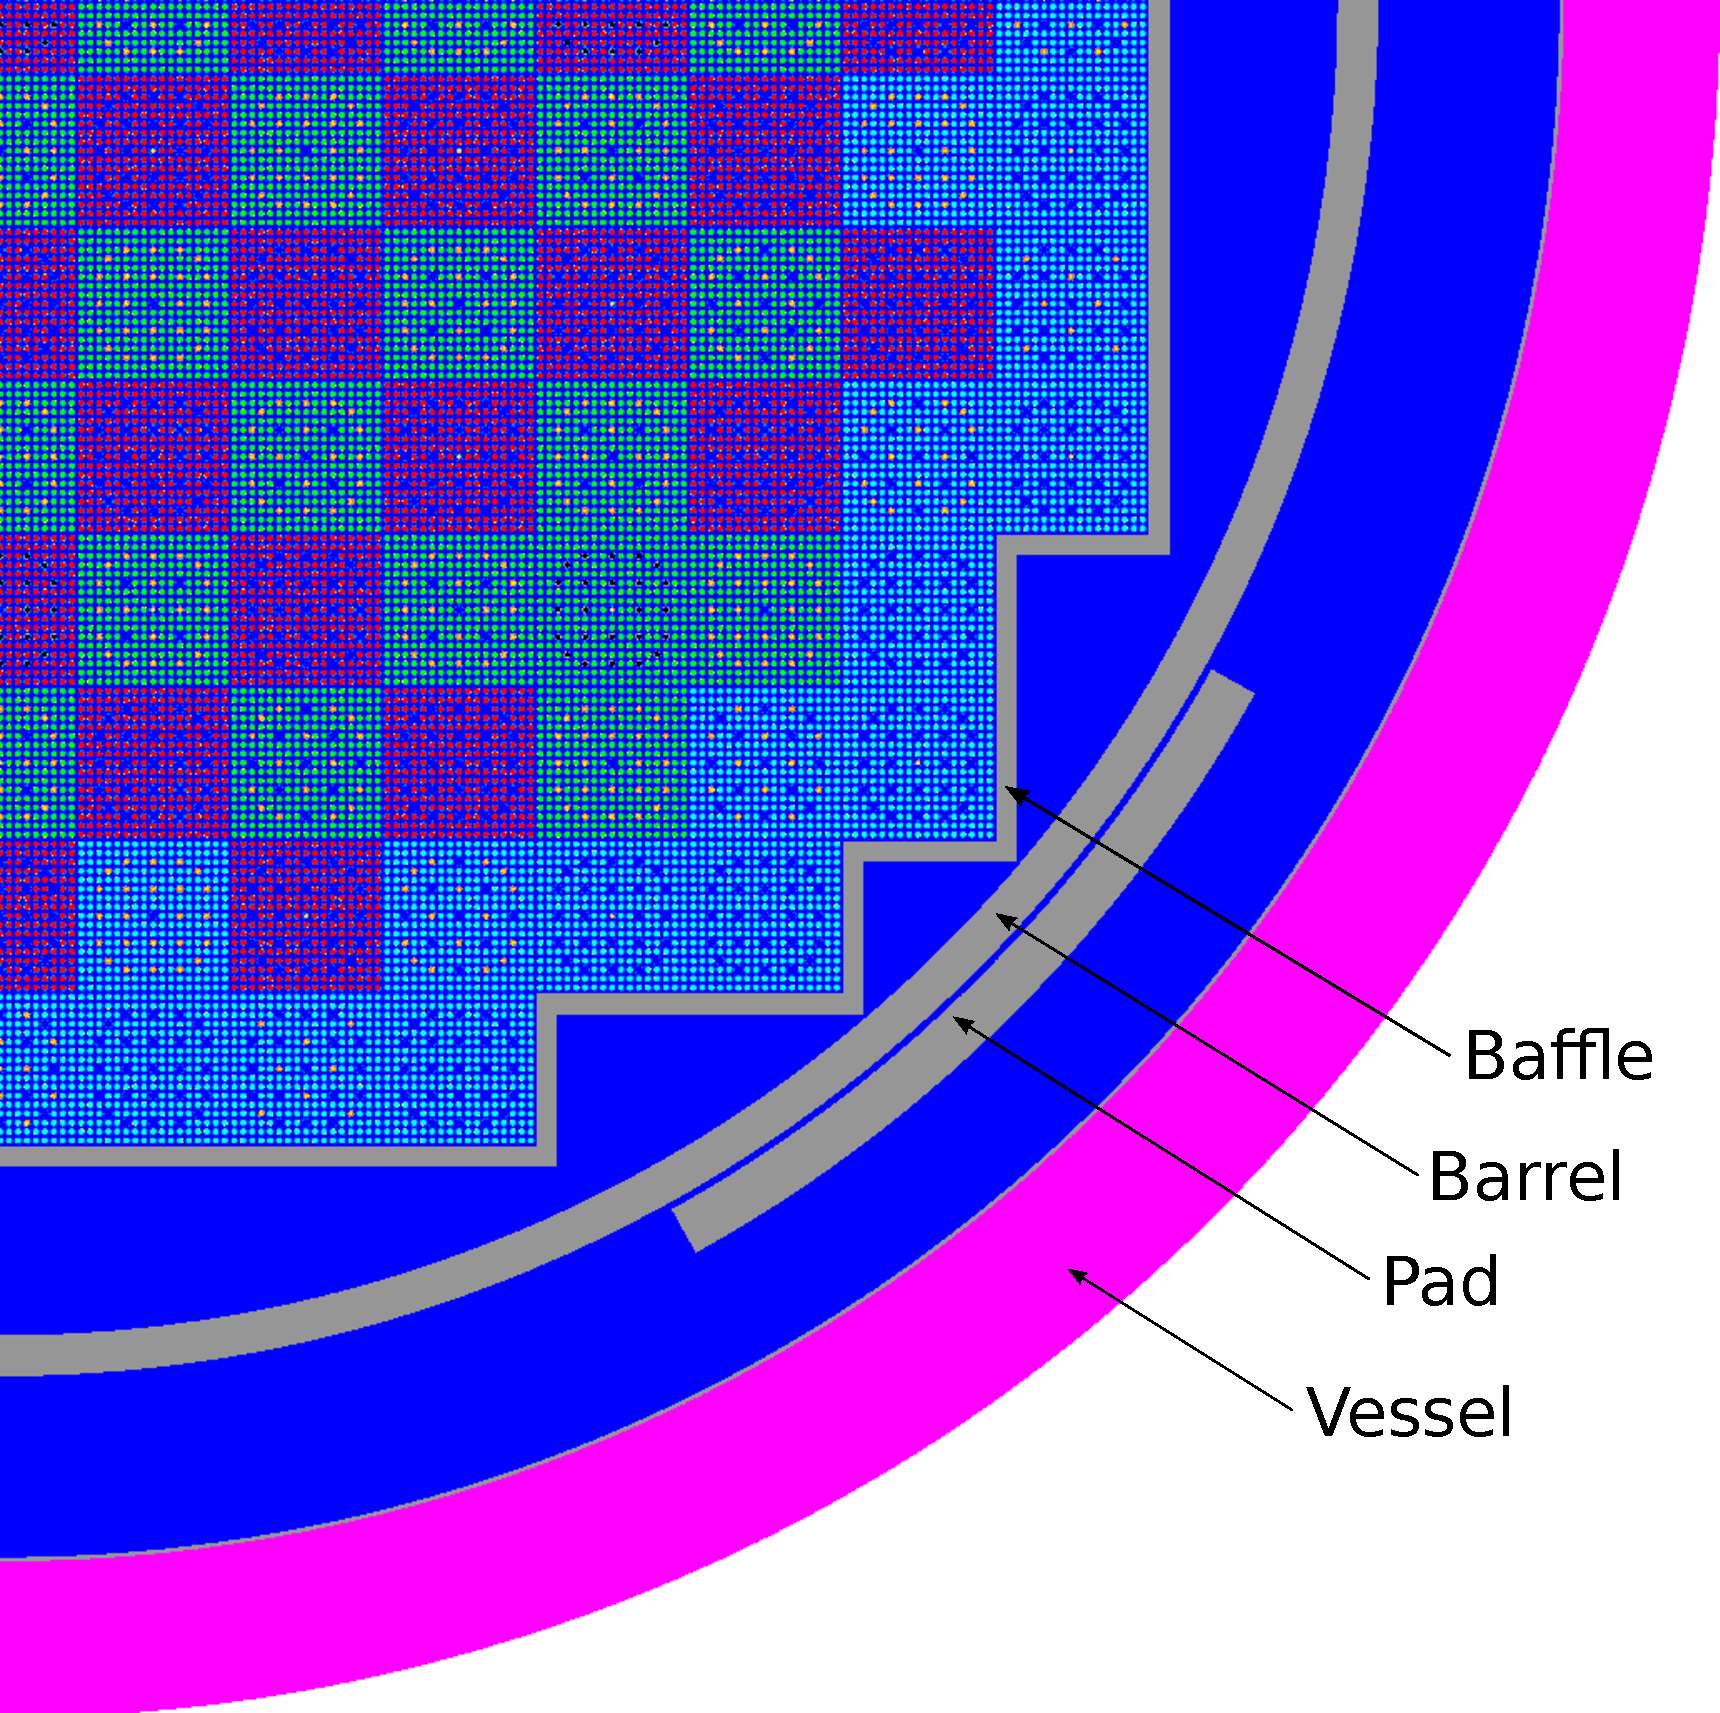
\includegraphics[width=5in]{figs/core_baffle.pdf}
\end{center}
\caption{\label{fig:corebaffle} Core baffle and vessel (image courtesy of Andrew Godfrey).}
\end{figure}

% fix: add figure showing exactly how the baffle gap is defined

The {\it baffle} is defined with a single material, the size of the gap between the
outer assembly and baffle, and the baffle thickness.
\begin{Verbatim}[fontsize=\small]

  baffle   SS304 0.19 1.26   ! material, gap (cm), and thickness (cm)

\end{Verbatim}

The barrel and vessel are defined with a {\it vessel} card. This card allows the
user to enter any arbitrary number of rings surrounding a core by specifying the
ring radii and the materials between the rings.

\begin{Verbatim}[fontsize=\small]

  vessel   mod 166.7 SS304 169.2 mod 175.0 SS304 176.0   ! materials and radii (cm)

\end{Verbatim}

There is currently no input defined to specify the neutron pad.

%%%%%%%%%%%%%%%%%%%%%%%%%%%%%%%%%%%%%%%
\subsubsection{Core Plates}

The core plates are large steel plates at the top and bottom of the core that have
various flow holes passing through them. All of the axial core heights are defined relative to the
top of the bottom core plate, and the total core {\it height} is defined as the distance
between the top of the bottom core plate and the bottom of the top core plate.

The core plates are modeled in the neutronics codes as smeared materials.
The upper and lower core plates are defined with a material composition, a thickness, and a
volume fraction of the structural material.
The remainder of the volume fraction is filled with coolant.

\begin{Verbatim}[fontsize=\small]

  lower_plate SS304  5.0  0.5   ! material, thickness (cm), volume fraction
  upper_plate SS304  7.6  0.5   ! material, thickness (cm), volume fraction
\end{Verbatim}

%%%%%%%%%%%%%%%%%%%%%%%%%%%%%%%%%%%%%%%
\subsubsection{Small Core Geometries}
\label{sec:smallcoregeom}

Even though the VERA input is designed for ``real'' core geometries, it can accommodate smaller
problems as well.
For example, to run a single-assembly calculation, the user would define the core size
as one assembly by one assembly, and all of the core maps would contain a single assembly.
\begin{Verbatim}[fontsize=\small]

  size 1                ! core composed of a single-assembly
  core_shape
     1

\end{Verbatim}

To model a single fuel rod, the user would define a core with one assembly and
an assembly with one rod in it.

